\documentclass{article}
\usepackage{float, amsmath}
\usepackage{graphicx} % Required for inserting images
\usepackage[margin=3cm]{geometry}
\usepackage{subfigure}
\usepackage{multicol, booktabs}

\title{\textbf{ISYE 6740 - Computational Data Analysis - \\ Final Project Report}}
\date{}

\begin{document}
\maketitle
\section*{}
    \textbf{Author}: Omar Masood \\
    \textbf{Project Title}: Topic Modeling of Religious Texts
\section{Problem Statement}
The \textit{Qur'an} claims to be the spiritual successor to the Old and New Testaments (\textit{Qur'an} 19:30). While historians, linguists, and religious scholars have examined these scriptures in an attempt to affirm or deny this claim, there are clear limits to human inspection alone. Topic modeling provides a useful and powerful new avenue by which we can examine these texts in their entirety to identify salient and common themes. Towards this goal, we employed three topic modeling techniques, Latent Dirichlet Allocation (LDA), BERTopic, and Top2Vec and applied them to English translations of the \textit{Qur'an}, the Old Testament, and the New Testament to identify topics from each text. We then compared both the outputs of these models as well as metrics such as perplexity, topic coherence, and topic diversity to determine which model performed best. There have been previous studies that examined the performance of various topic modeling techniques\footnote{Egger, R. and Yu, J., A Topic Modeling Comparison Between LDA, NMF, Top2Vec, and BERTopic to Demystify Twitter Posts, \textit{Front. Sociol.}, https://doi.org/10.3389/fsoc.2022.886498} and single topic models on religious texts.\footnote{Alshammeri, M., Atwell, E., Alsalka, M.A. (2021). Quranic Topic Modeling Using Paragraph Vectors. \textit{Intelligent Systems and Applications}} This project aims to combine these approaches and answer two questions: \begin{enumerate}
    \item Are there similarly detectable themes across the \textit{Qur'an}, the Old Testament, and New Testament?
    \item Which method performs best for topic modeling religious texts?
\end{enumerate}

\section{Data Sources}
    All the data were open source and can be found via multiple sources online dedicated to providing high-quality English translations of the \textit{Qur'an}, Old Testament, and New Testament. Each dataset was a .csv file where each row represented a verse. The \textit{Qur'an} has a total of 6,236 verses, the Old Testament has a total of 23,145 verses, and the New Testament has a total of 7,958 verses. 
 
\section{Methodology}
    \subsection{Data Preprocessing}
    While our BERTopic and Top2Vec models do not necessarily require substantive text pre-processing, we needed to ensure that the data were in a usable state for our LDA model. We relied on the \textit{spacy}, \textit{nltk}, and \textit{gensim} packages for text pre-processing. The main steps of this involved 1) casting all words to lowercase, 2) retrieving the lemma of each word, and 3) removing common stopwords as defined by \textit{nltk}. This provided a list of verses from each text in their lemmetized, or base, form. At this stage, the data were ready to be passed in to BERTopic and Top2Vec models. For our LDA model, we then passed our data through \textit{sklearn}'s TfidfVectorizer to retrieve a matrix of TF-IDF (term frequency-inverse document frequency) features for each text. TF-IDF is a measure which captures the importance of words (inverse document frequency) and the frequency of those words (term frequency):
    \begin{equation*}
        TF \cdot IDF(t, d) = \frac{\text{frequency that term } t \text{ appears in document } d}{\text{Total number of terms in } d} \cdot \log(\frac{\text{Total number of documents } N}{\text{Number of documents which contain } t})
    \end{equation*}
    Our vectorizer scored unigrams, bigrams, and trigrams, which was necessary given the nature of the texts which often contain short phrases whose component terms may have been meaningless as unigrams.
    \begin{figure}[H]
        \centering
        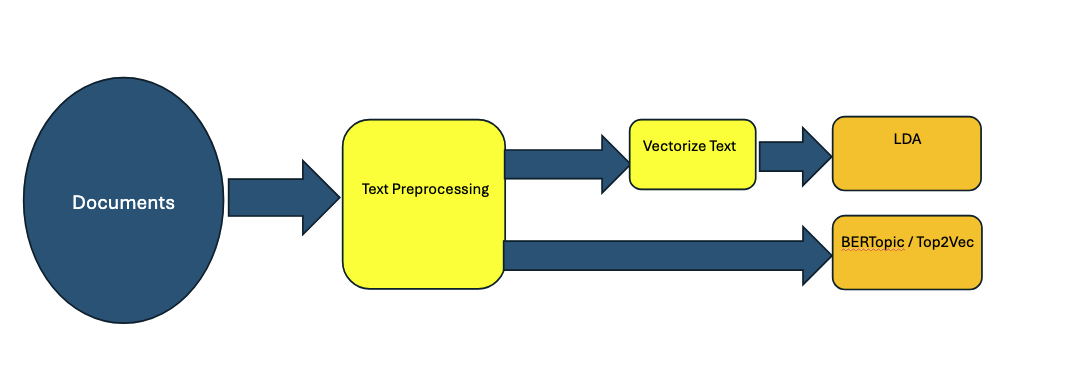
\includegraphics[width=1\linewidth]{Diagram.png}
        \caption{Data Processing}
    \end{figure}

    \subsection{LDA}
        Latent Dirichlet Allocation (LDA) is a bag-of-words model that determines the probability a word is associated with a topic and the probability that a topic is associated with a word. It then assigns topics to a document based on its contents (i.e., the words). To achieve the best performance, we tuned our LDA model using random search cross-validation with topic coherence as our scoring metric. We tuned the following hyperparameters: \textit{batch\_size}, \textit{learning\_offset}, \textit{learning\_decay}, \textit{doc\_topic\_prior}, \textit{n\_components}. We found that our LDA model performed best when the number of topics (\textit{n\_components}) was 7 and our $\alpha$ parameter was high, to indicate documents are made up of several topics.
        
    \subsection{BERTopic \& Top2Vec}
        BERTopic models use BERT (Bidirectional Encoder Representations from Transformers) embeddings and sentence transformers to create topics from texts. Sentence transformers convert our input text into uniform length vectors. As opposed to LDA, which focuses on the frequency of terms, BERTopic models benefit from being able to detect the context within text by modifying the TF-IDF calculation and generating a c-TF-IDF score (class-based Term Frequency-Inverse Document Frequency). c-TF-IDF is able to better identify important terms by computing the importance of terms within a cluster of documents. Somewhat similarly to BERTopic, Top2Vec creates jointly embedded document and word vectors, documents are mapped on an \textit{n}-dimensional space and clustered with other similar documents and/or documents with distinctive wording. 
        
        Both BERTopic and Top2Vec models rely on UMAP and HDBSCAN for dimensionality reduction and clustering, respectively. We tuned UMAP and HDBSCAN models and passed them into our BERTopic and Top2Vec models. Both models benefited from allowing smaller cluster size and using cluster reduction. We relied on BERTopic and Top2Vec's topic reduction, both of which use HDBSCAN to cluster similar topics and combine them. The main difference between our BERTopic and Top2Vec model parameters was the decision to use a Doc2Vec embedding in our Top2Vec model which significantly improved the performance of our model. Doc2Vec creates a unique vector representation for each document in our dataset. We determined a Doc2Vec embedding model was most appropriate due to specialized nature of our text data. 
        
    \subsection{Challenges and Limitations}
        There were some challenges and limitations inherent in our data. The \textit{Qur'an} is both a poetic and prosaic text, whose contents vacillate between narration and legislation. The \textit{Qur'an} also has a uniquely repetitive structure, where phrases are often repeated throughout the text. The latter is also a feature of the Old and New Testament. Another challenge was the fact that the Old Testament has more than three times the number of verses than both the \textit{Qur'an} and the New Testament. As a result, the models trained on Old Testament data typically performed better in one or all metrics. 

\section{Evaluation and Final Results}
    Our primary means of evaluating the LDA, BERTopic, and Top2Vec models was the topic coherence score, available through \textit{gensim}. Topic coherence is a measure of how well a topic is supported by the text in it. Specifically, we used the Cv (Coefficient of Topic Coherence) measure, which somewhat proxies human interpretation. However, as BERTopic and Top2Vec models are not based on topic-word distributions, topic coherence is not sufficient to assess our models' performances. To address this, we also compared topic diversity. Topic diversity measure the distinctiveness of the different topics. The results of our models are below. 
    \subsection{LDA}
    As stated above, we setup our LDA models to generate seven topics. All three of our models had middling topic coherence and diversity scores, as shown in Table 1, indicating sub-optimal performance. As we can see, terms such as 'allah,' 'lord,' 'prophet,' 'people' appear across several topics. This is most likely a result of LDA representing documents as a bag-of-words - the more frequently appearing terms are in most if not all of our topics. We experimented with different \textit{max\_df} values between 0.1 and 0.9 in our TF-IDF vectorizer. Using lower values of \textit{max\_df} ignores terms which appear across several documents. However, even when considering terms with low document frequency, the LDA was not able to create topics with discernible meaningfulness or distinctiveness.     
    \begin{table}[H]
        \centering
        \begin{tabular}{|c|c|c|c|c|}
            \hline
             & Topic Coherence & Perplexity & Topic Diversity & Num. of Topics \\
            \hline
            Quran & 0.4 & 2406.4 & 0.657 &7\\
            \hline 
            Old Testament & 0.38 & 1221 &0.57&7\\
            \hline
            New Testament & 0.31 & 1940&0.6&7\\
            \hline 
        \end{tabular}
        \caption{LDA metrics}
        \label{tab:my_label}
    \end{table}
    \begin{figure}[H]
        \centering
        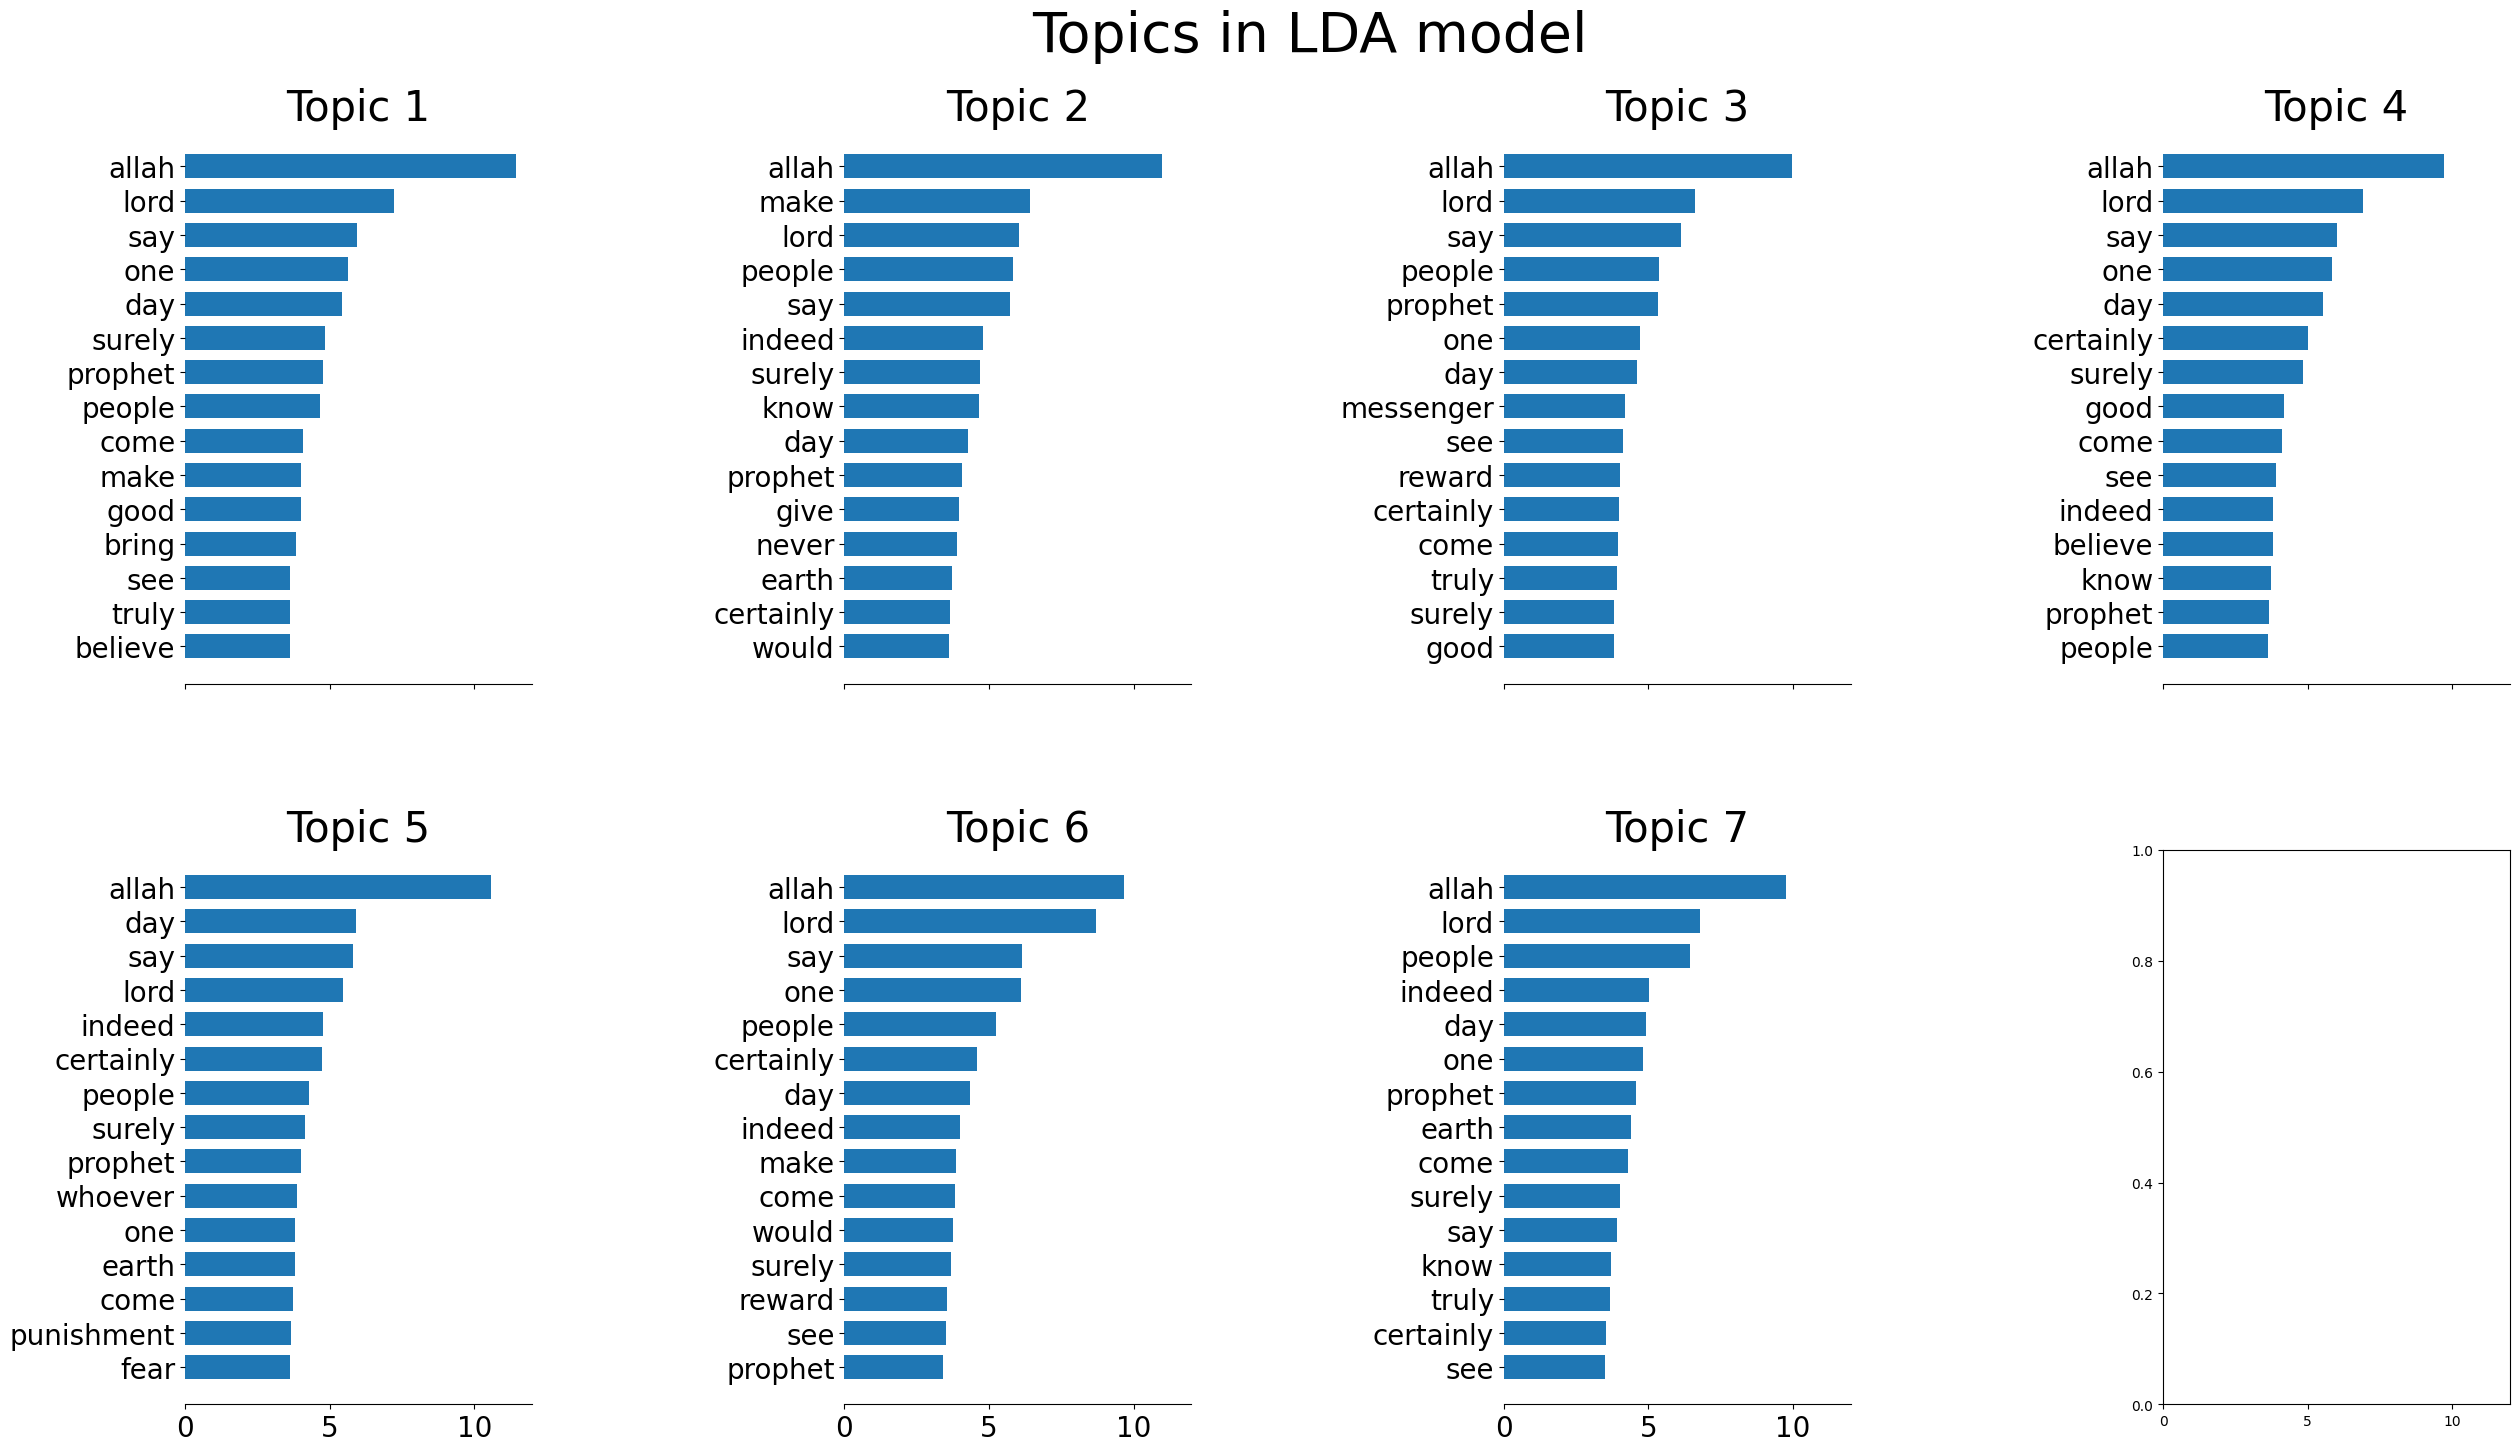
\includegraphics[width=1.1\linewidth]{QuranLDA.png}
        \caption{Quran LDA Topic Modeling}
        \label{fig:enter-label}
    \end{figure}
    
\subsection{BERTopic}
    Our BERTopic model performed much better than the LDA model, both in regard to topic coherence and diversity scores but also qualitatively in generating meaningful topics. As seen in Table 2 below, we can see a marked improvement in both metrics. As BERTopic and Top2Vec are not probabilistic models, we do not report perplexity as it is not a meaningful metric. \\
    In Figure 3, we display a sample of eight topics our model generated from \textit{Qur'an} data, the total number of topics generated is captured in Table 2. As we can see, our topics are are much more distinctive with clearly identifiable themes, and topics 3, 4, and 8 are especially noteworthy. Those familiar with the biblical narrative will recognize Topic 3 as the story of \textbf{Moses} and the Egyptian \textbf{pharaoh}. Topic 8 captures to the story of \textbf{Joseph}, his jealous \textbf{brothers} and doting \textbf{father}, as well as Joseph's prescient \textbf{dreams}. Topic 4 captures the twin epithets of Muhammed, who is regarded as both God's \textbf{prophet} and \textbf{messenger} in the \textit{Qur'an}.  
    
    \begin{table}[H]
            \centering
            \begin{tabular}{|c|c|c|c|}
                \hline
                 & Coherence & Topic Diversity & Num. Topics\\
                \hline
                Quran & 0.78&0.96&45\\
                \hline 
                Old Testament & 0.8&0.89&25\\
                \hline
                New Testament & 0.77&0.93&34\\
                \hline 
            \end{tabular}
            \label{tab:my_label}
            \caption{BERTopic metrics}
        \end{table}
    
    \begin{figure}[H]
        \centering
        \subfigure[Quran Topic Word Scores]{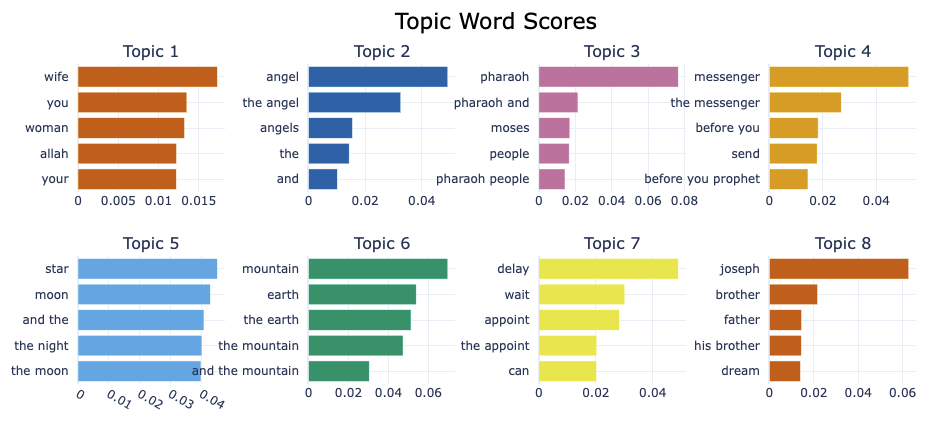
\includegraphics[width=1\linewidth]{quranbertbar.png}}
        \caption{BERTopic Word Scores}
        \label{fig:enter-label}
    \end{figure}

    We can compare a sampling of the topics produced by our BERTopic models to see if they find similar topics between the \textit{Qur'an} and the Old Testament, and the \textit{Qur'an} and the New Testament. The table below shows topics that were identified as similar based on cosine similarity. Each row shows a topic from our BERTopic model trained on the \textit{Qur'an} and a similar topic from the models trained on the Old Testament and New Testament respectively, based on their cosine similarity. The cosine similarity determines likeness based on the the dot product of two vectors, normalized by product of the Euclidean distance of the two vectors. See equation 1, where $Vec_A$ and $Vec_B$ represent the topic vectors.
    \begin{equation}
        cos(\theta) = \frac{Vec_A \cdot Vec_B}{||Vec_A|| \cdot ||Vec_B||}
    \end{equation}
    In Table 2, cells with \textit{No Match} mean the \textit{Qur'an} topic was matched to the topic indexed at the 0 index, which we can interpret as there being no match. The 0 index topic is a catch all for terms not placed in any other topic. We see that the topics produced by the BERTopic model appear to be internally consistent, however, there were few corresponding topics from our Old Testament model. We were able to match topics much more successfully between the \textit{Qur'an} and the New Testament BERTopic models.\\
    
    \begin{table}[H]
        \centering
        \begin{tabular}{|p{1cm}|p{4cm}|p{4cm}|p{4cm}|}
        \toprule
        Topic & Quran & Old Testament & New Testament \\
        \midrule
        2 & ['mountain', 'earth', 'the earth', 'the mountain', 'and the mountain'] & \textit{No Match} & ['ship', 'the ship', 'wind', 'they', 'ship and'] \\
        3 & ['joseph', 'brother', 'he', 'father', 'his brother'] & \textit{No Match} & ['joseph', 'jacob', 'son joseph', 'joseph and', 'the son joseph'] \\
        4 & ['they', 'they will', 'will', 'then', 'their'] & ['wheel', 'wing', 'one', 'face', 'their'] & ['garment', 'his', 'he', 'hand', 'and'] \\
        5 & ['burn', 'fire', 'hellfire', 'the hellfire', 'flame'] & \textit{No Match} & ['light', 'darkness', 'the light', 'light the', 'the light the'] \\
        6 & ['create', 'drop', 'sperm drop', 'sperm', 'from'] & \textit{No Match} & ['labour', 'work', 'labour and', 'you', 'every man'] \\
        7 & ['fruit', 'tree', 'palm tree', 'palm', 'olive'] & ['locust', 'the locust', 'caterpiller', 'the', 'the caterpiller'] & ['tree', 'fruit', 'fig', 'fig tree', 'forth'] \\
        8 & ['drink', 'water', 'pure wine', 'boiling', 'wine'] & ['they', 'but they', 'they have', 'their', 'not'] & ['water', 'thirst', 'woman samaria', 'drink', 'give drink'] \\
        9 & ['favour will', 'lord favour will', 'favour will you', 'lord favour', 'your lord favour'] & \textit{No Match} & ['and', 'the', 'that', 'they', 'be'] \\
        10 & ['warner', 'news', 'deliverer', 'deliverer good', 'deliverer good news'] & \textit{No Match} & ['and', 'the', 'that', 'they', 'be'] \\
        11 & ['reminder', 'the reminder', 'this reminder', 'reminder and', 'surely this reminder'] & \textit{No Match} & ['remembrance', 'remembrance the', 'timotheus', 'call remembrance the', 'always remembrance'] \\
        \bottomrule
        \end{tabular}
        \caption{BERTopic Matching}
        \label{tab:my_label}
    \end{table}
    
\subsection{Top2Vec}
    Our Top2Vec performed well in creating meaningful and distinctive topics, far better than our LDA models. As Table 4 shows, it generates topics with high diversity. 
    \begin{table}[H]
            \centering
            \begin{tabular}{|c|c|c|c|}
                \hline
                 &  Coherence & Topic Diversity &Num. Topics$^*$\\
                \hline
                Quran & 0.38&0.86&50\\
                \hline 
                Old Testament & 0.5&0.95&30\\
                \hline
                New Testament & 0.4&0.81&35\\
                \hline 
            \end{tabular}
            \caption{Top2Vec metrics}
            \label{}
             $^*$The number of topics were reduced using hierarchical topic reduction to the number specified in the table above. 
    \end{table}
    
    Top2Vec provides a built-in function to generate a word cloud of terms associated with a topic. One example is provided below, for a single topic from the \textit{Qur'an}. From the example below, we can see that our Top2Vec model generated a topic pertaining to the forbiddance of polytheism and association of any other entities with God in Islam. 
    \begin{figure}[H]
        \centering
        \subfigure[Quran Wordcloud Topic 1]{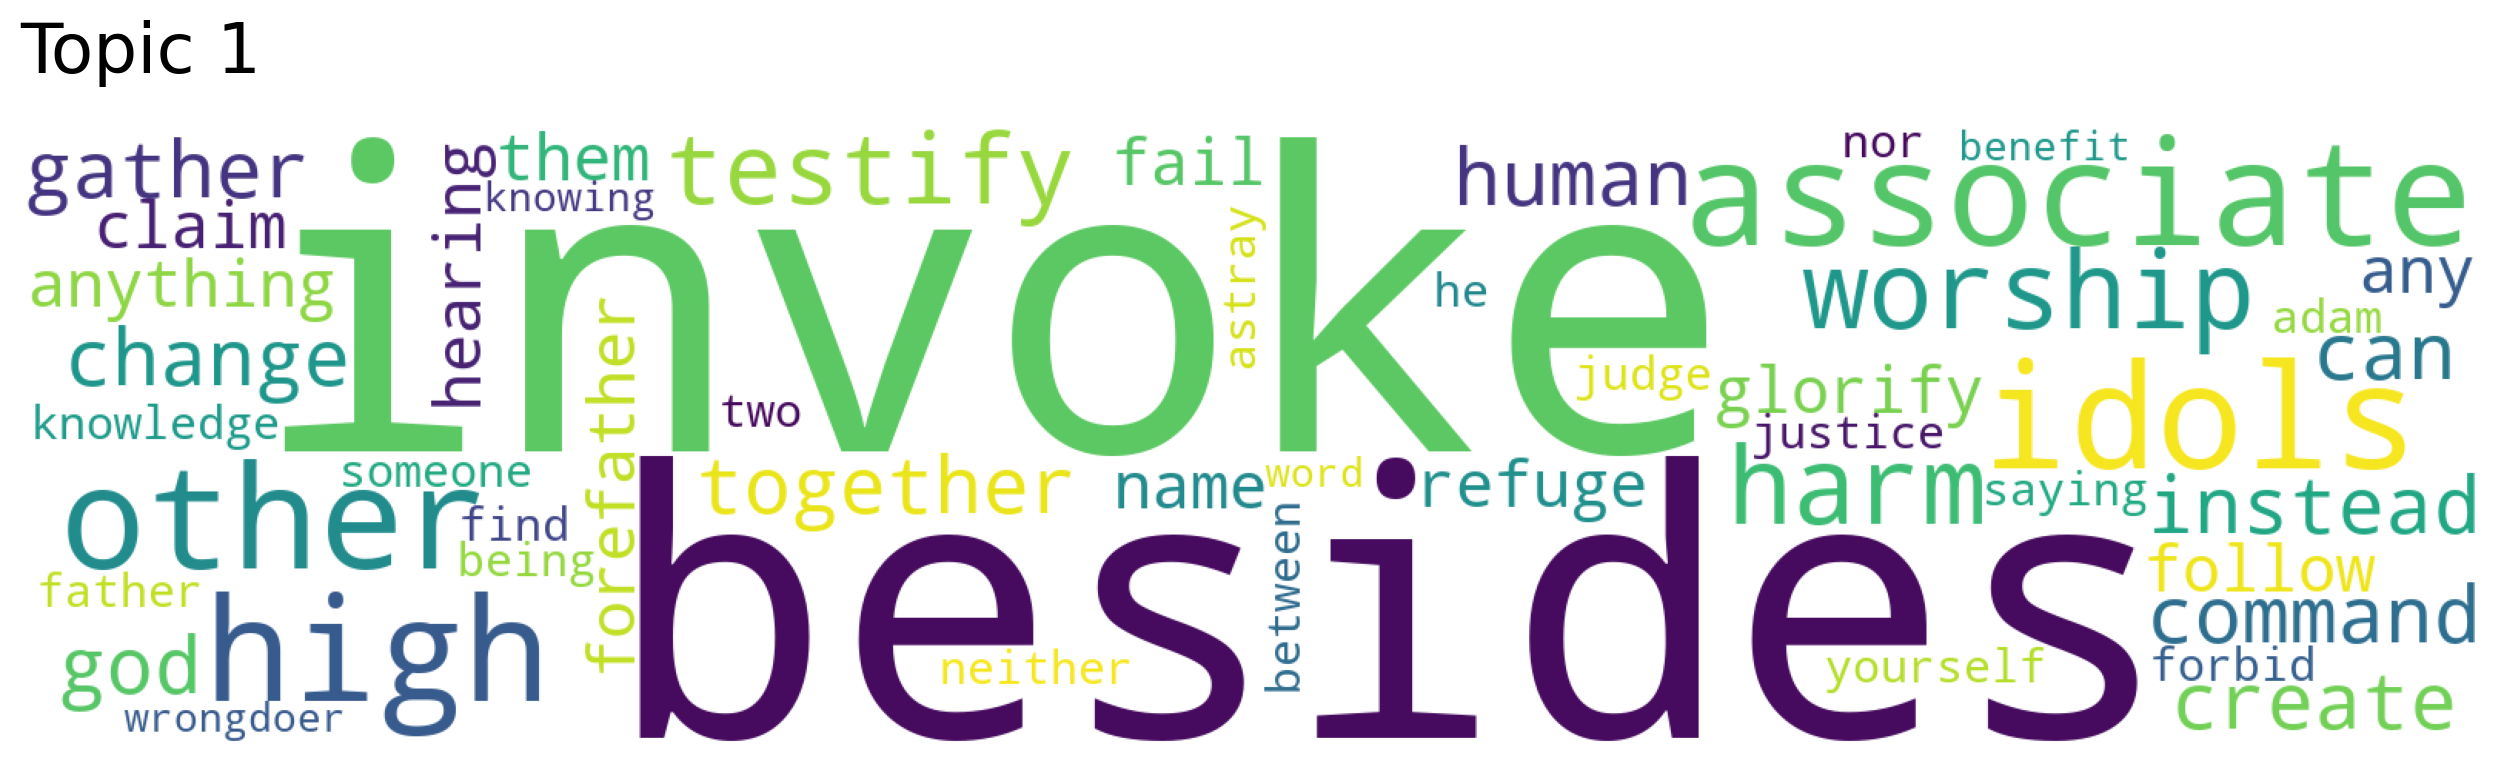
\includegraphics[width=0.65\linewidth]{quranwordcloud1.png}}
    \end{figure}

    We can also visualize the classification of all verses. We passed our data through a different UMAP model and reduced the dimensionality of topic embeddings to be able to display it as a scatterplot. Figure 4 shows the distribution of topics for the \textit{Qur'an}, similar representations for the Old and New Testament can be found in the Appendix. 
    \begin{figure}[H]
        \centering
        \subfigure[]{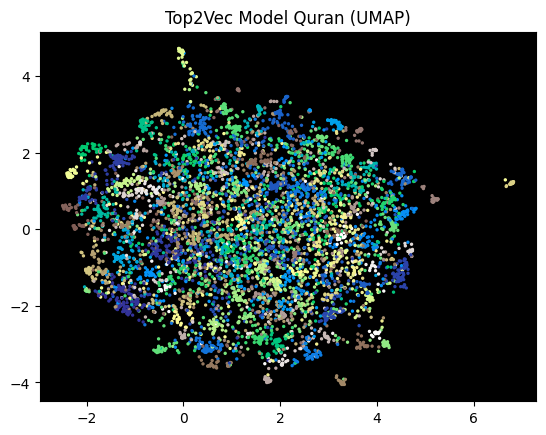
\includegraphics[width=0.85\linewidth]{QuranUMAP.png}}
        \caption{UMAP Top2Vec Representation}
        \label{fig:enter-label}
    \end{figure}

    As we did with our BERTopic models, we can match topics from our Top2Vec model trained on the text of the \textit{Qur'an} to topics from our Old Testament and New Testament models based on cosine similarity. As Table 5 shows, topics from our Quran-trained BERTopic model were matched with topics in the Old and New Testament models. However, it is difficult to intuitively understand why these topics were considered similar.\\

    \begin{table}[H]
        \centering
        \begin{tabular}{|p{1cm}|p{4cm}|p{4cm}|p{4cm}|}
        \toprule
        Topic & Quran & Old Testament & New Testament \\
        \midrule
        2 & ['reduce' 'resurrect' 'doubt' 'bad' 'enjoyment' 'mary' 'fact' 'inform'
         'really' 'simply'] & ['precept' 'language' 'chapiter' 'pomegranate' 'eli' 'row' 'philistine' 'yield' 'shiloh' 'scarlet'] & ['james' 'simon' 'peter' 'mary' 'weep' 'disciple' 'philip' 'john' 'sepulchre' 'tribe'] \\
         \hline
        3 & ['wait' 'deliver' 'too' 'clearly' 'keep' 'message' 'unless' 'family'
         'reject' 'free'] & ['sihon' 'heshbon' 'amorites' 'graven' 'image' 'arnon' 'grove' 'breach' 'bashan' 'joram'] & ['loud' 'angel' 'earth' 'sea' 'heaven' 'gather' 'voice' 'sun' 'cloud' 'sound'] \\
         \hline
        4 & ['testify' 'pharaoh' 'against' 'every' 'prevail' 'drown' 'two' 'plead'
         'her' 'parent'] & ['precept' 'language' 'chapiter' 'pomegranate' 'eli' 'row' 'philistine' 'yield' 'shiloh' 'scarlet'] & ['go' 'ship' 'depart' 'galilee' 'country' 'judaea' 'multitude' 'thence'  'side' 'besought'] \\
         \hline
        5 & ['belong' 'heaven' 'whatever' 'alone' 'earth' 'almighty' 'wise' 'all'
         'capable' 'heavens'] & ['vineyard' 'plant' 'grape' 'inhabit' 'yield' 'vine' 'sow' 'fruit' 'desolate' 'branch'] & ['wash' 'rebuke' 'foot' 'peter' 'immediately' 'marvel' 'eye' 'peace' 'cry' 'multitude'] \\
         \hline
        6 & ['sun' 'moon' 'mountain' 'sky' 'everything' 'earth' 'create' 'heaven'
         'night' 'capable'] & ['town' 'pestilence' 'famine' 'sword' 'scatter' 'suburb' 'drive' 'reproach' 'leah' 'psaltery'] & ['wash' 'rebuke' 'foot' 'peter' 'immediately' 'marvel' 'eye' 'peace' 'cry' 'multitude'] \\
         \hline
        7 & ['change' 'find' 'high' 'intend' 'woman' 'man' 'adam' 'forgiving'
         'transgress' 'disobey'] & ['duke' 'blind' 'just' 'instruction' 'corrupt' 'korah' 'knowledge' 'wickedness' 'iniquity' 'merciful'] & ['sepulchre' 'wind' 'sea' 'ship' 'go' 'straightway' 'run' 'depart' 'third' 'side'] \\
         \hline
        8 & ['put' 'destine' 'trust' 'around' 'side' 'definitely' 'should' 'hypocrite' 'delay' 'hasten'] & ['town' 'pestilence' 'famine' 'sword' 'scatter' 'suburb' 'drive' 'reproach' 'leah' 'psaltery'] & ['sepulchre' 'wind' 'sea' 'ship' 'go' 'straightway' 'run' 'depart' 'third' 'side'] \\
         \hline
        9 & ['seven' 'ear' 'darkness' 'cover' 'capable' 'strike' 'victory' 'at' 'eye' 'sea'] & ['innocent' 'believe' 'carcass' 'daniel' 'watch' 'wonder' 'dream'
         'toucheth' 'abhor' 'cloud'] & ['believeth' 'offer' 'ashamed' 'sacrifice' 'obtain' 'once' 'gift' 'last' 'charge' 'conscience'] \\
         \hline
        8 & ['oath' 'lot' 'something' 'garden' 'family' 'mother' 'example' 'story'
         'thamud' 'parent'] & ['babylon' 'jehoiakim' 'bury' 'reign' 'isaiah' 'judah' 'zedekiah' 'jerusalem' 'jeremiah' 'hananiah'] & ['loud' 'angel' 'earth' 'sea' 'heaven' 'gather' 'voice' 'sun' 'cloud' 'sound'] \\
         \hline
        9 & ['invoke' 'associate' 'besides' 'idols' 'astray' 'god' 'worship'
         'consider' 'claim' 'instead'] & ['statute' 'observe' 'incline' 'commandment' 'keep' 'walk' 'precept' 'law'
         'you' 'judgment'] & \textit{No Match} \\
         \hline
        \bottomrule
        \end{tabular}
        \caption{Topic Matching}
        \label{tab:my_label}
    \end{table}
    

\subsection{Results}

By evaluating our models' metrics as well as qualitative analysis of the generated topics, we see that our LDA model performed relatively poorly in modeling topics in the \textit{Qur'an}. However, this is not unexpected given the challenges we discussed above. We see similar results for LDA models using Old Testament and New Testament verses in Figure 5 (see Appendix), the repetition of terms seems to confound our LDA models and produce topics with little meaning. Our LDA models scored significantly lower than our BERTopic model in both topic coherence and topic diversity. We can also see that our BERTopic and Top2Vec models produce topics that are more meaningful and discernibly distinct. While our Top2Vec models have low topic coherence scores, this may in part be explained by the fact that coherence is an imperfect measure for Top2Vec due to the fact that \textit{gensim} calculates coherence using a bag-of-words model. 

It is clear that LDA is unable to appropriately ignore certain frequently appearing corpus terms, which makes it ill-suited for topic modeling complex texts such as religious scripture. Top2Vec and BERTopic modeling produced better performing models, with much more meaningful topics. In partiuclar, BERTopic especially was able to generate topics with high topic coherence and diversity. Additionally when comparing topics across models, our BERTopic models were able to generate topics which were matched to topics from other models that made intuitive sense. These factors indicate that BERTopic may be the best method for the specialized task of topic modeling highly specialized texts. 

The questions as to whether there are similar detectable themes across the \textit{Qur'an}, the Old Testament, and the New Testament remains open. Both our BERTopic models and Top2Vec models were able to match Quran topic to topics in the Old and New Testament. However, in the latter case, the topics generated by our Top2Vec model which were matched did not seem thematically similar. This suggests that further work is needed to determine a more appropriate measure, rather than cosine similarity to determine likeness between topics. Our BERTopic models produced more encouraging results (see Table 3), albeit there were fewer matches across the topics from our models.  

\pagebreak
\section{Appendix}
\subsection{LDA}
    \begin{figure}[H]
        \centering
        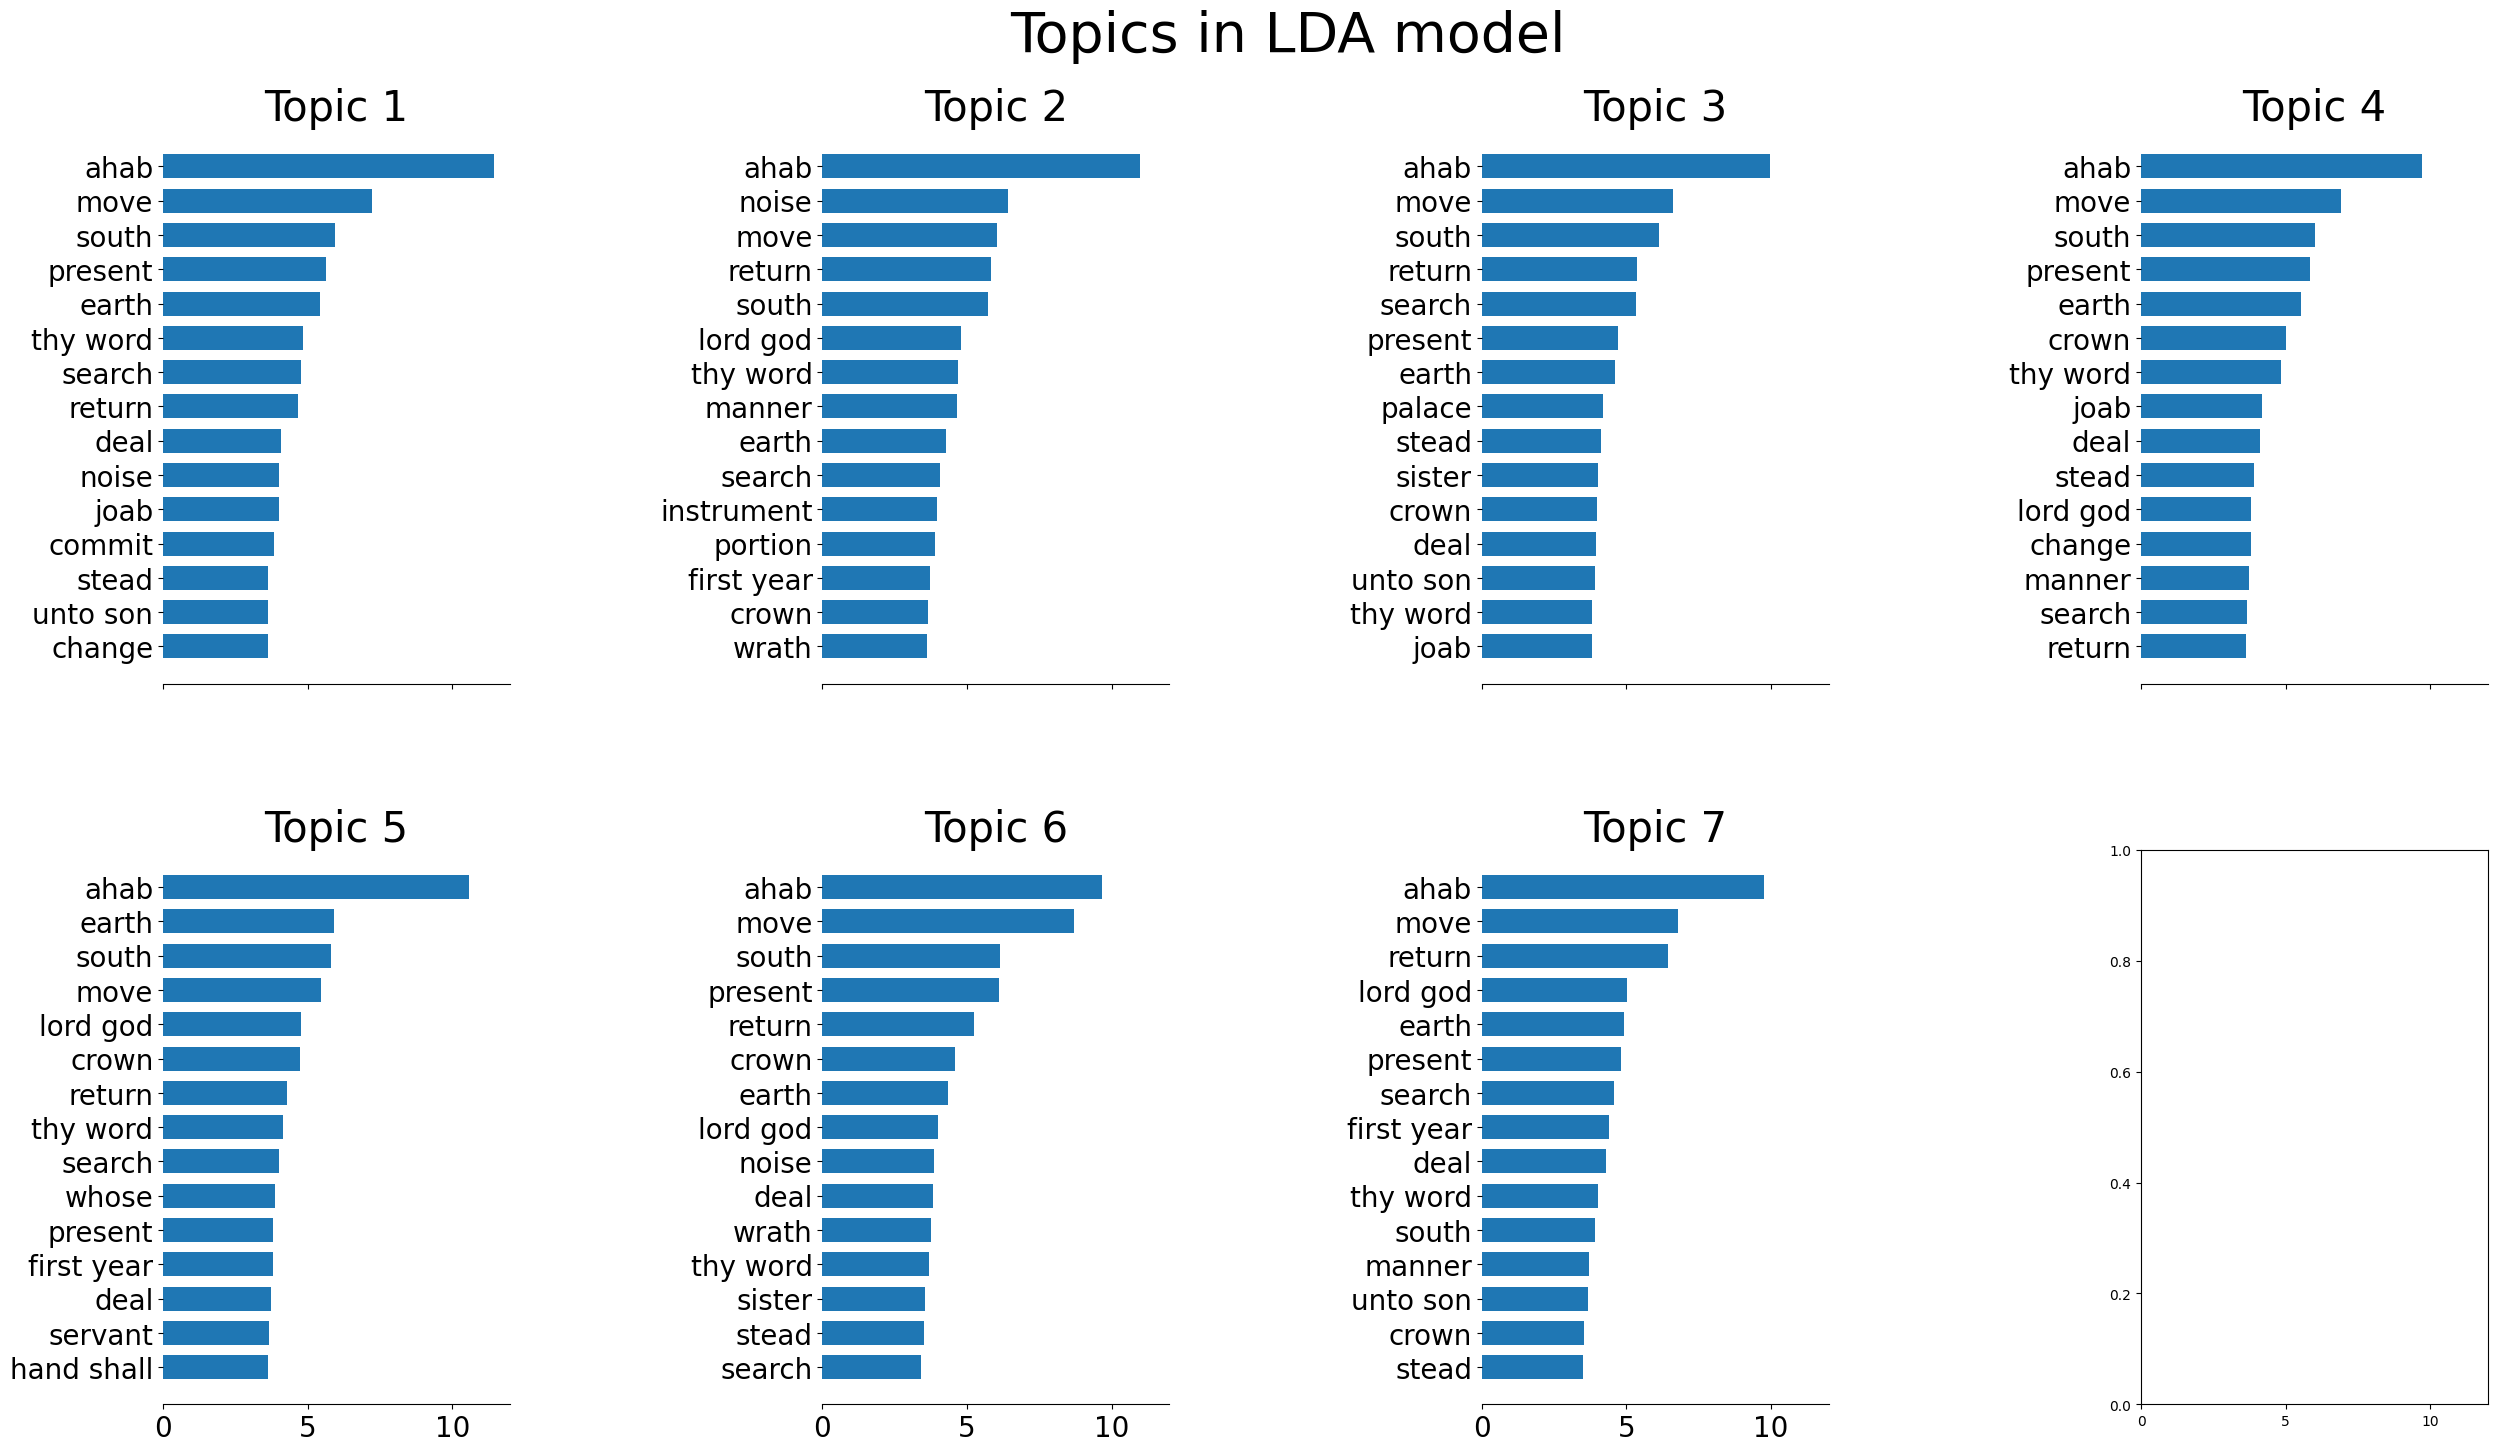
\includegraphics[width=0.9\linewidth]{OldTLDA.png}
        \caption{Old Testament LDA Topic Modeling}
        \label{fig:enter-label}
    \end{figure}
    \begin{figure}[H]
        \centering
        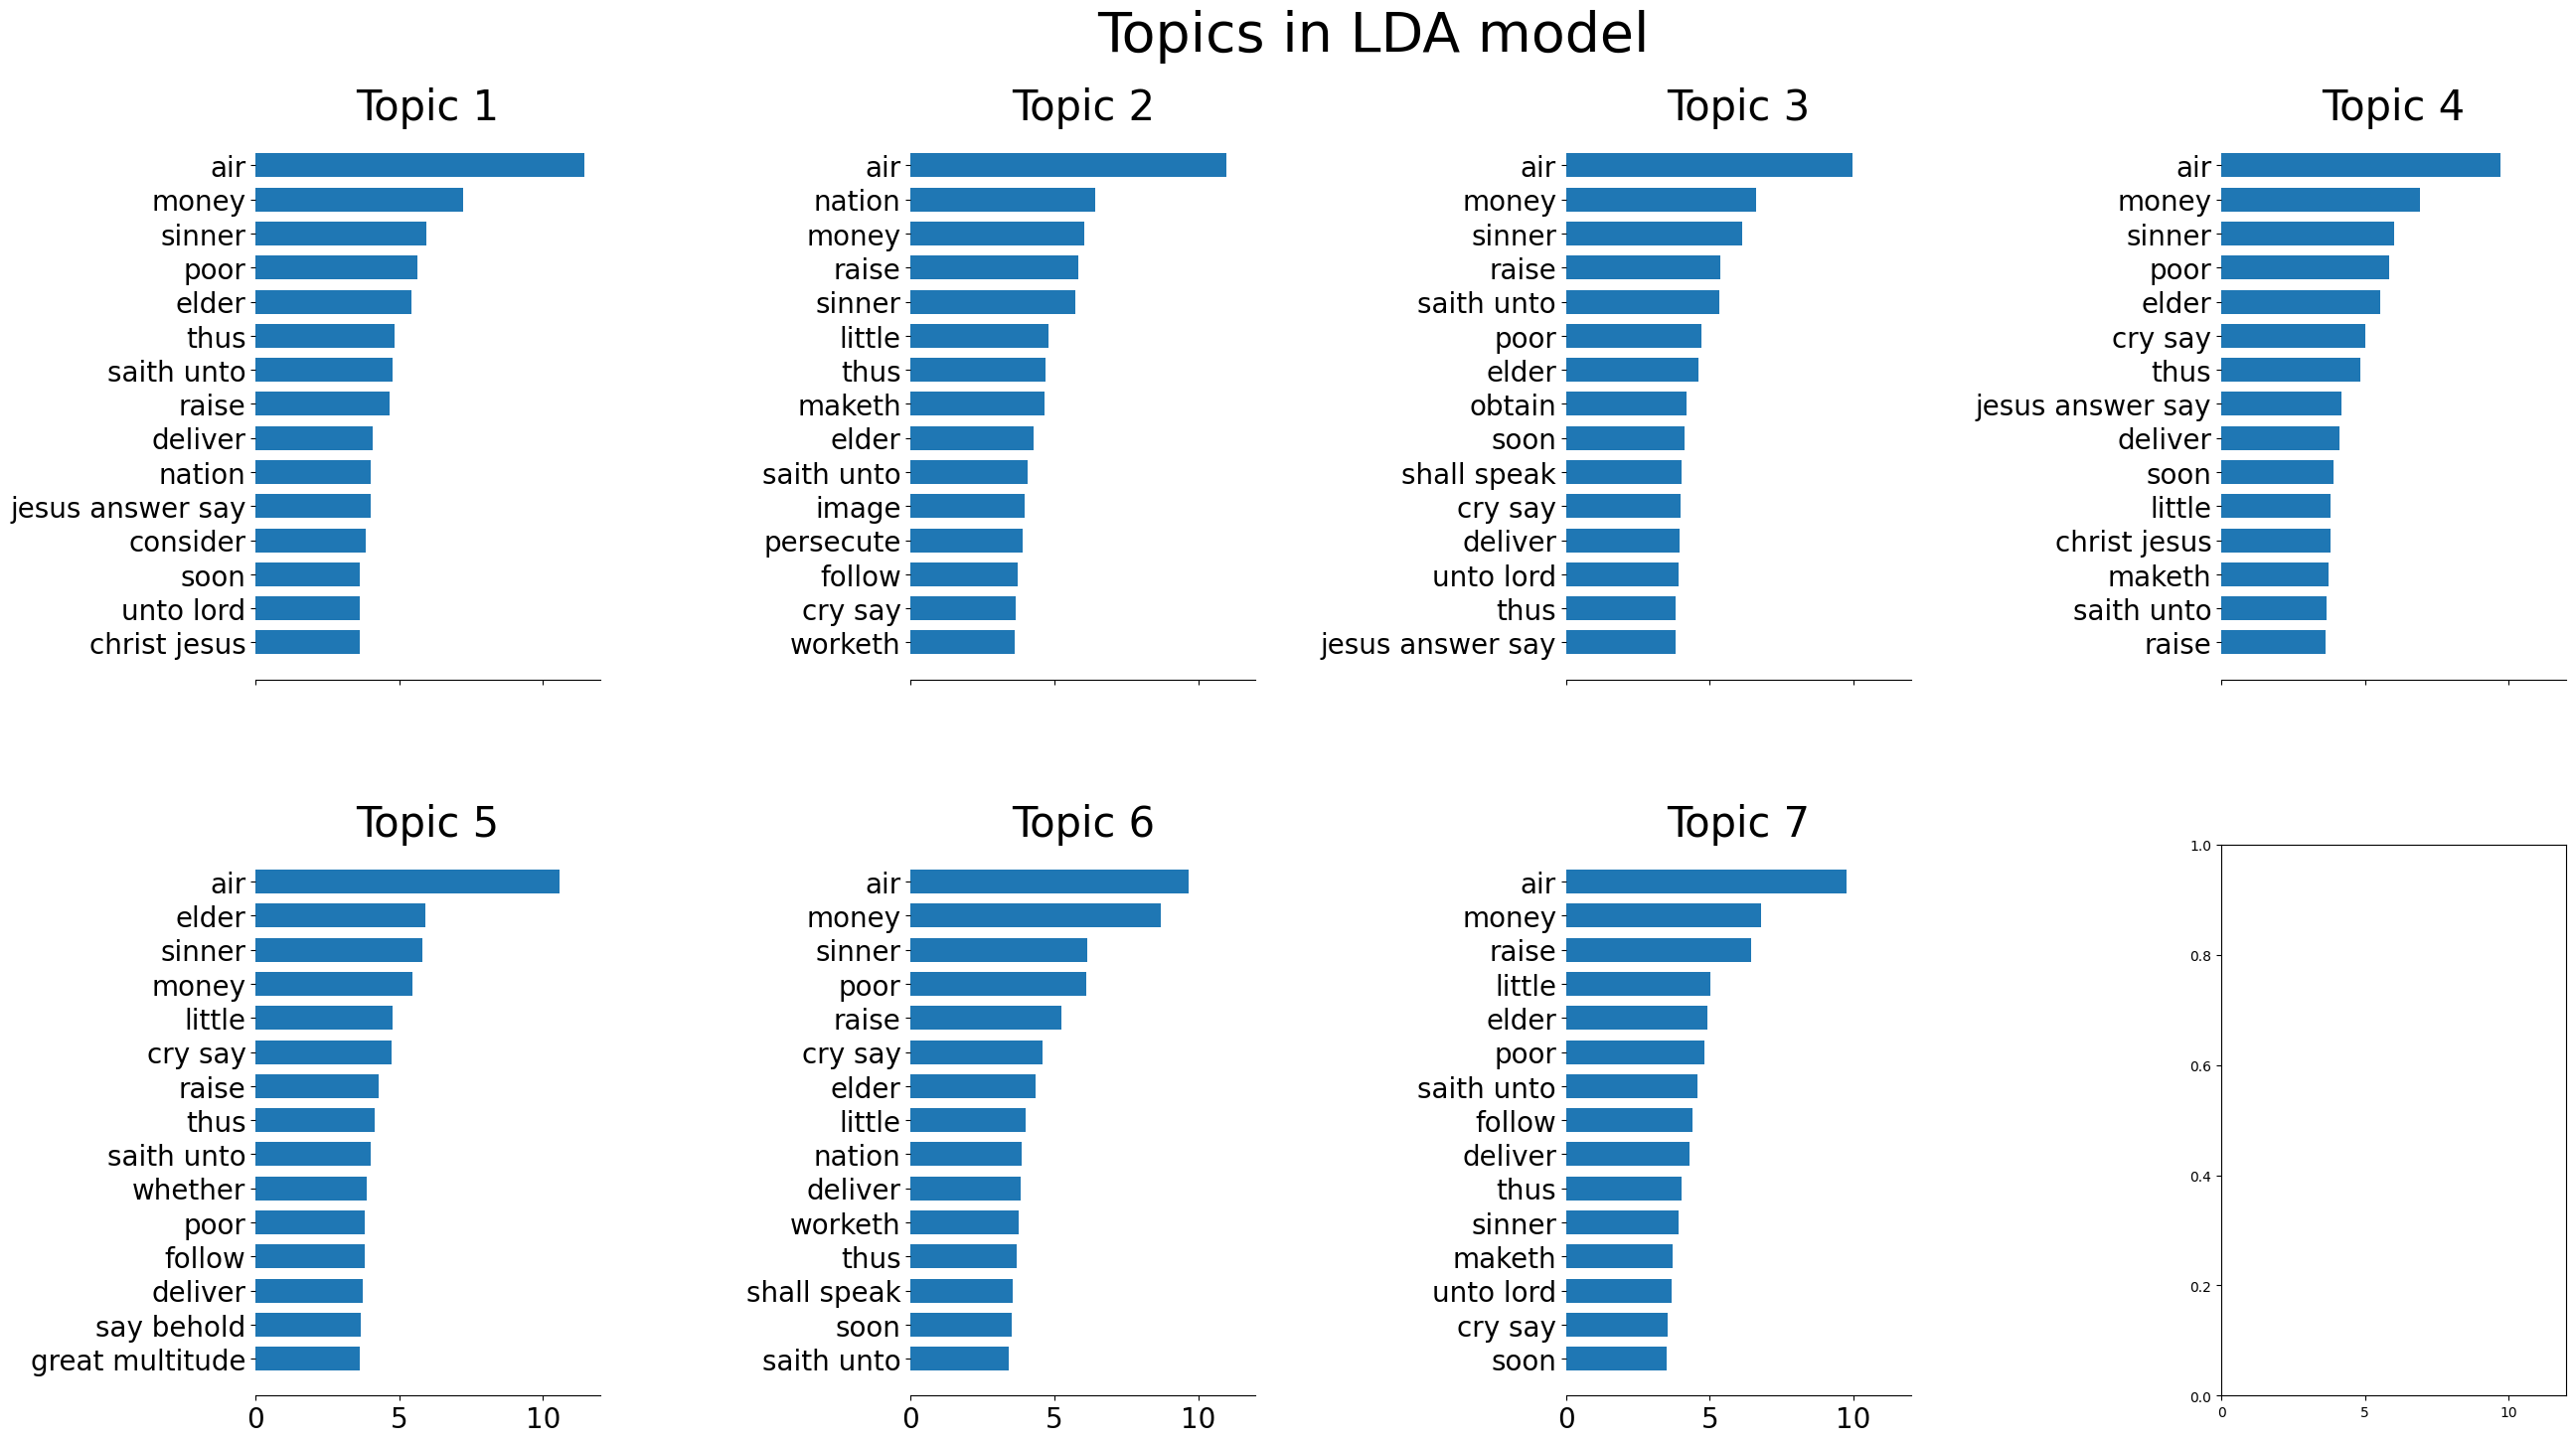
\includegraphics[width=0.9\linewidth]{NewTLDA.png}
        \caption{New Testament LDA Topic Modeling}
        \label{fig:enter-label}
    \end{figure}
\subsection{BERTopic}
    \begin{figure}[H]
        \subfigure[Old Testament Topic Word Scores]{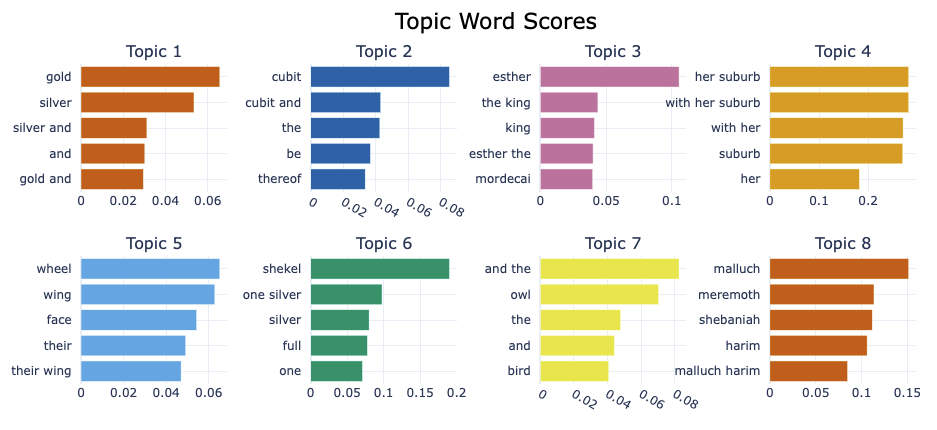
\includegraphics[width=1\linewidth]{oldtbertbar.png}}
        \subfigure[New Testament Topic Word Scores]{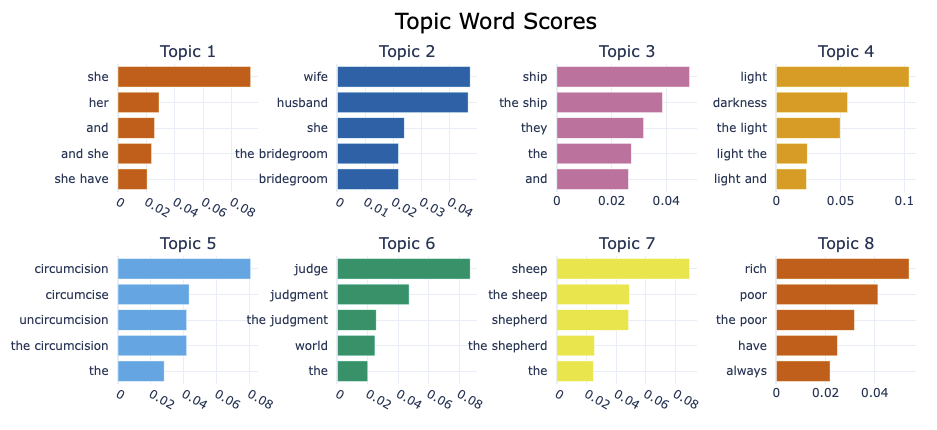
\includegraphics[width=1\linewidth]{newtbertbar.png}}
        \caption{BERTopic Word Scores}
        \label{fig:enter-label}
    \end{figure}
\subsection{Top2Vec}
    
    \begin{figure}[H]
        \subfigure[]{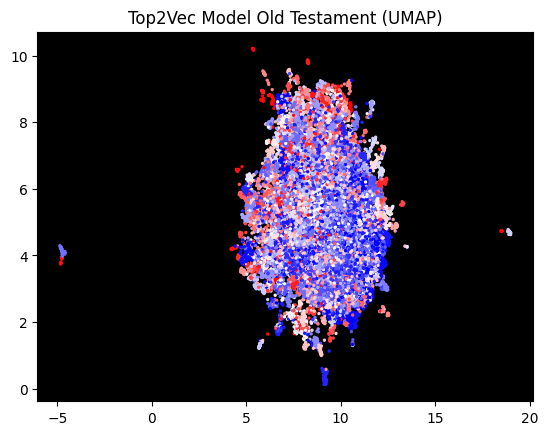
\includegraphics[width=0.6\linewidth]{OldTUMAP.png}}
        \subfigure[]{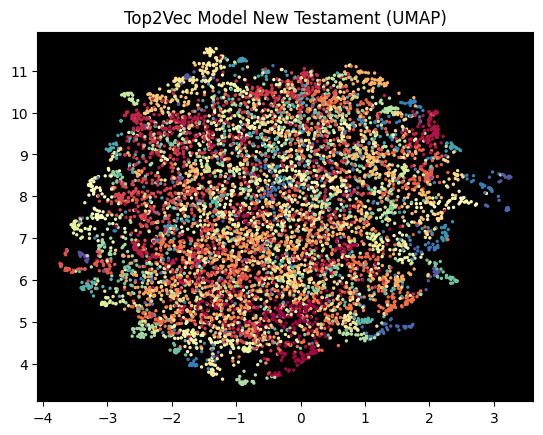
\includegraphics[width=0.6\linewidth]{NewTUMAP.png}}
        \caption{UMAP Representation}
        \label{fig:enter-label}
    \end{figure}
    \begin{figure}[H]
        \subfigure[Old Testament Wordcloud Topic 1]{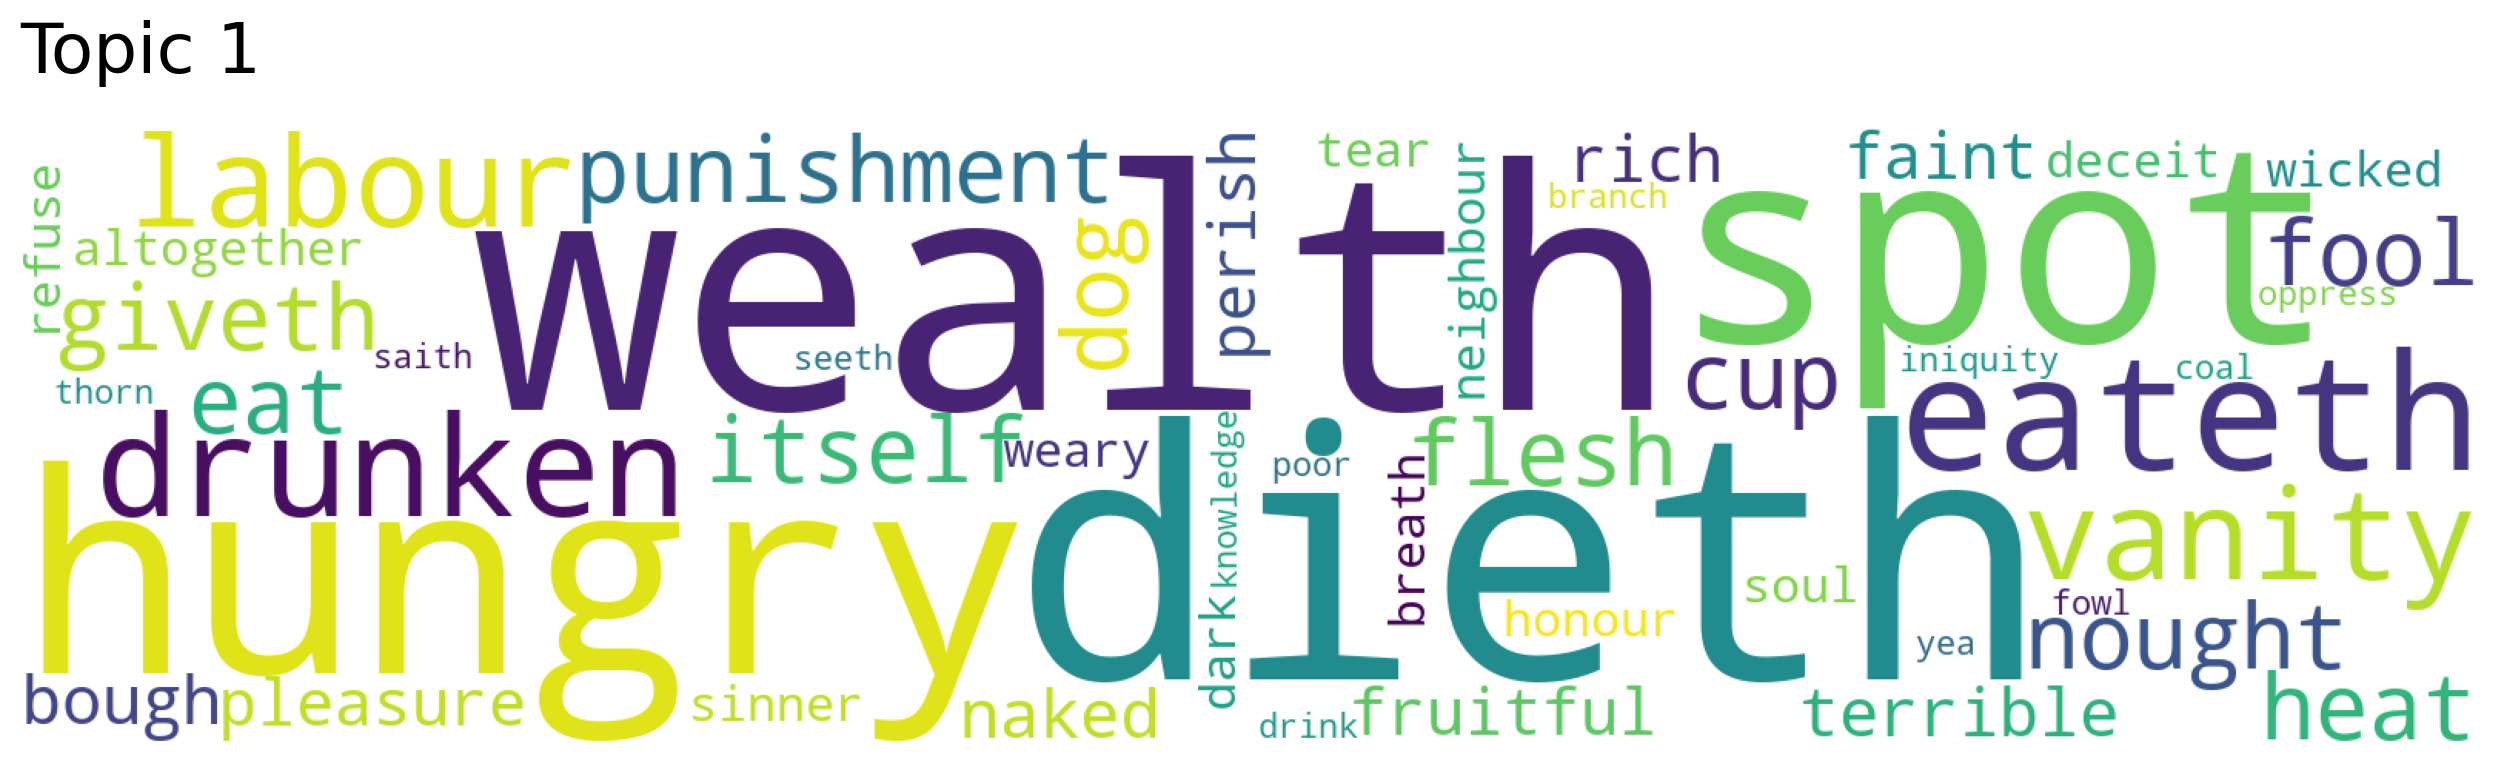
\includegraphics[width=0.55\linewidth]{oldtwordcloud1.png}}
        \subfigure[New Testament Wordcloud Topic 1]{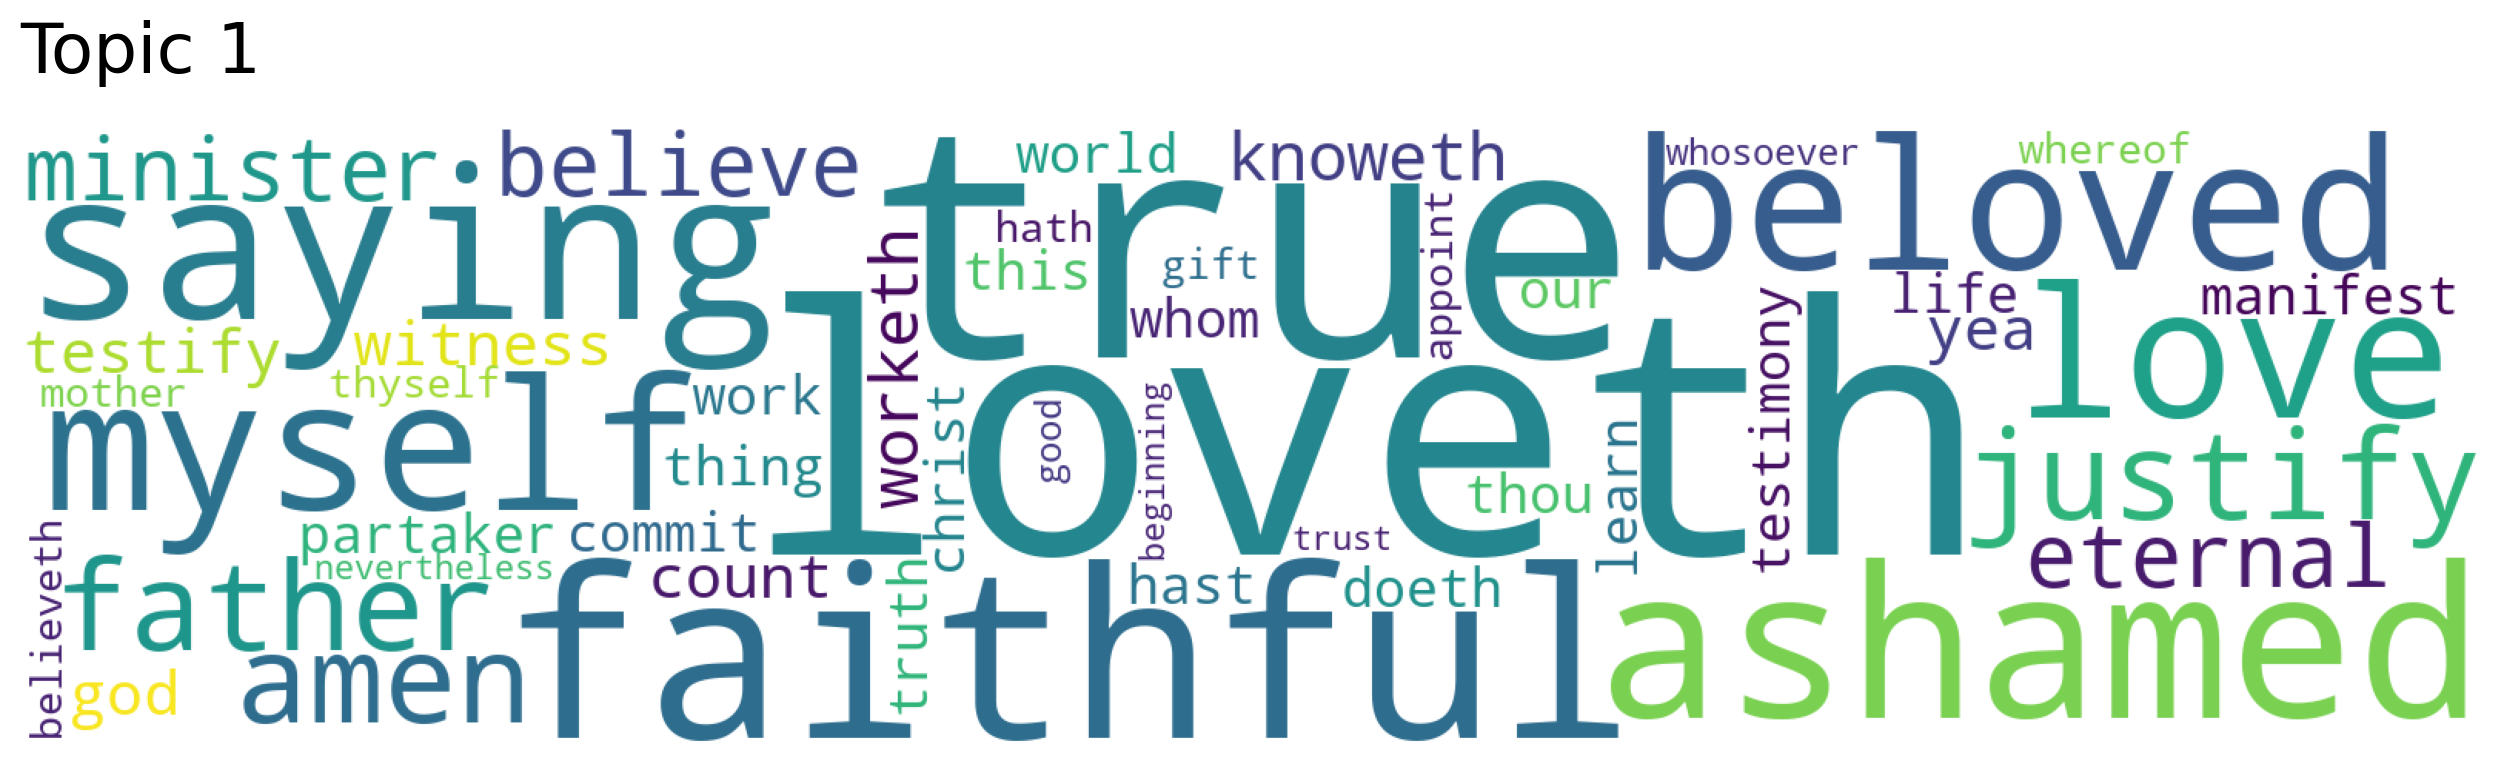
\includegraphics[width=0.55\linewidth]{newtwordcloud1.png}}
        \caption{Topic Word Clouds}
        \label{fig:enter-label}
    \end{figure}
\end{document}
